%% Author_tex.tex
%% V1.0
%% 2012/13/12
%% developed by Techset
%%
%% This file describes the coding for rsproca.cls

\documentclass[]{rsos}%%%%where rsos is the template name

\usepackage{lineno}
\linenumbers

\usepackage[T1]{fontenc}
\usepackage[utf8]{inputenc}

% For Pandoc highlighting needs

% Pandoc citation processing

\usepackage{float}
\usepackage{booktabs}
\newcommand{\beginsupplement}{ \setcounter{table}{0}     \renewcommand{\thetable}{S\arabic{table}}\setcounter{figure}{0} \renewcommand{\thefigure}{S\arabic{figure}}}

%%%% *** Do not adjust lengths that control margins, column widths, etc. ***

%%%%%%%%%%% Defining Enunciations  %%%%%%%%%%%
\newtheorem{theorem}{\bf Theorem}[section]
\newtheorem{condition}{\bf Condition}[section]
\newtheorem{corollary}{\bf Corollary}[section]
%%%%%%%%%%%%%%%%%%%%%%%%%%%%%%%%%%%%%%%%%%%%%%%

\begin{document}

%%%% Article title to be placed here
\title{Combination of field and experimental data together with computational models reveal cognitive mechanisms behind cleaner fish behaviour}

\author{
Andrés E. Quiñones$^{1}$,
Zegni Triki$^{2}$,
Redouan Bshary$^{1}$}

\address{
  $^{1}$Institute of Biology, University of Neuchâtel, Neuchâtel, Switzerland\\
  $^{2}$Department of Zoology, Stockholm University, Stockholm, Sweden}
%%%% Subject entries to be placed here %%%%
\subject{
Behavioural ecology,
Cognitive ecology,
Animal behaviour}

%%%% Keyword entries to be placed here %%%%
\keywords{
learning,
cleaners,
behaviour,
bayesian statisitics,
mutualism}

%%%% Insert corresponding author and its email address}
\corres{
  AE. Quiñones\\
  e-mail: \href{mailto:andreseqp@gmail.com}{\nolinkurl{andreseqp@gmail.com}}
}

%%%% Abstract text to be placed here %%%%%%%%%%%%
\begin{abstract}
While it is generally straightforward to quantify individual performance in cognitive experiments, identifying the underlying cognitive processes remains a major challenge. Often, different mechanistic underpinnings may yield similar performances, and Lloyd Morgan's cannon warrants acceptance of the simpler explanation. Alternatively, when the different mechanisms interact with environmental conditions, variation in performance across environments might allow to statistically infer the mechanism responsible. However, to do this it is necessary to have quantitative predictions for the different candidate mechanisms. Here, we use a set of computational models to get quantitative predictions from alternative learning mechanisms, and using Bayesian statistics fit the model parameters to performance data. We used experimental data on performance in an ephemeral reward task by wild-caught cleaner fish Labroides dimidiatus, as well as cleaner and client fish densities from the locations of capture. The task can in principle be solved by estimating future consequences of an action, or by perceiving the removal of the ephemeral reward as psychological punishment (negative reinforcement). We found that a model where cleaners only estimate the future consequences of their actions explains best which cleaner relative abundances cause the fish to develop a preference for an ephemeral food source. This model also yields performances that can be considered the result of locally optimal decision-rules, in contrast to the negative reinforcement model. We argue that the combination of computational models with data is a powerful tool to infer the mechanistic underpinning behind cognitive performance.
\end{abstract}
%%%%%%%%%%%%%%%%%%%%%%%%%%%

%% Some pieces required from the pandoc template
\providecommand{\tightlist}{%
  \setlength{\itemsep}{0pt}\setlength{\parskip}{0pt}}
\providecommand{\EndFirstPage}{%
}

\maketitle

\hypertarget{introduction}{%
\subsection{Introduction}\label{introduction}}

Cooperation among individuals of the same or different species is
ubiquitous in nature. Whenever such interactions involve some degree
of partner choice, biological market theory predicts that the exchange
rate of goods and/or services traded adjusts to the law of supply and demand
\citep{noe_Biological_1995a}. While biological market models have largely focused
on evolutionary time scales \citep{noe_Biological_1994a, johnstone_Mutualism_2008a}
\(\color{red}{\text{Hoekstra xxxx}}\), supply and demand conditions, which typically
depend on the abundance of the species involved, certainly vary in time
and space within ecological time scales. Therefore, natural selection should
favour the ability to flexibly adjust decisions and behavioural output to
current market conditions. Indeed, such adjustments have been repeatedly
documented \citep{axen_Signalling_1996}. In animals, an obvious general candidate
mechanism for the strategic adjustment is the cognitive machinery. However,
it is not clear which cognitive mechanisms allow individuals to adjust their
behaviour to the varying market conditions. As adjustments to changes in
market conditions have been documented in a great variety of species with
highly variable brain anatomies, the question arises to what extent mechanisms
beyond basic associative learning may be involved.

One example of strategic adjustment in a biological market is the marine
cleaning mutualism involving the cleaner fish \emph{Labroides dimidiatus} and
`client' fish. Clients offer themselves as food patches for cleaners to
remove ectoparasites, which gives the cleaners calories and the clients
improved health \citep{waldie_LongTerm_2011, ros_Does_2011, triki_Effects_2016}. As cleaners have about 2000
interactions per day \citep{grutter_Relationship_1995}, they regularly face
the situation that two clients seek cleaning simultaneously. In such
conditions, it is important to distinguish between `resident' and
`visitor' client species \citep{bshary_Cleaner_2001a}. The residents have
small home ranges and hence access to only the local cleaner, while the
visitors have large home ranges and hence access to two or more
cleaners. Thus, visitors have the option to switch to another cleaner if
being made to wait, while residents must wait for inspection. Indeed,
visitors have been observed to use their partner choice options in that
way \citep{bshary_Choosy_2002}, which may explain why cleaners give
visitors service priority in a field study in the Red Sea
\citep{bshary_Cleaner_2001a}. More generally, cleaners apparently prefer to
interact with visitors \citep{triki_Marine_2021}. Such a preference may be
linked to a client's value as a food patch; visitors are on average
larger than residents \citep{bshary_Cleaner_2001a}, and size is positively
correlated with parasite load \citep{grutter_Relationship_1995a}. However,
early laboratory experiments showed that leaving causes service
priority independent of client value \citep{bshary_Asymmetric_2002}.
The experiments consisted of asimultaneous two-choice task,
where cleaners had to decide which of two
Plexiglas plates, which offered equal amounts of food, to approach first
and eat mashed prawn of it. One plate was made to behave like a
resident, i.e.~it would remain until the cleaner had eaten off it. The
other plate was made to behave like a visitor, i.e.~it would be removed
if not inspected first. Cleaners learned to prefer the visitor plate and
hence obtained the double amount of food \citep{bshary_Asymmetric_2002}.
Adult cleaner fish outperform various primates as well as rats and
pigeons in this original version of the biological market task
\citep{salwiczek_Adult_2012, zentall_Early_2017}; only African grey
parrots solve this task as well \citep{pepperberg_Can_2014}. As the correct
solution must be learned, and primates are known to readily distinguish
between one and two reward units if presented in more conventional ways
\(\color{red}{\text{ref}}\), what makes the task difficult for most non-cleaners?

Recent research on the cognitive tool kit needed to solve an ephemeral
reward task has used a broad approach as proposed by Shettleworth
\citep{shettleworth_Cognition_2009},
who defined cognition as includes all ways in which animals take in information
through the senses, process, retain and decide to act on it. Indeed, perception
of relevant cues is of major importance for individual performance;
i.e.~what relevant information is encoded in the design of the two
plates (colour versus size; \citep{wismer_Cuebased_2019}), or whether
the information is in the colour of
the food \citep{pretot_Comparative_2021, pretot_Comparing_2016}, and
whether the food is visible or hidden/released only when the subjects
made choices on a touch screen \citep{pretot_Factors_2016}. However, identifying
cues as salient is not the only challenge of the ephemeral reward task,
as revealed by proximate learning models. Such models allow varying the
cognitive tool kit and to evaluate which minimal kit is necessary to solve
the task at hand (e.g. \citep{dubois_Model_2021}). Applied to the ephemeral
reward task, learning models showed that basic reinforcement learning does
not suffice to solve the task \citep{prat_Modelling_2022, quinones_Reinforcement_2019}.
This is particularly so when models assume the more complex natural
situation in which cleaners not only face resident-visitor pairs but also
visitor-visitor and resident-resident pairs, as well only a resident or
only a visitor. To be able to give visitors priority over residents,
cleaners need to be able to assess a client's value separately for the
three possible forms of encounter (alone, paired with a fish with the
same strategic option, paired with a fish with the alternative strategic option)
\citep{quinones_Reinforcement_2019}. The ability to keep such separate scores
for the same stimulus has been termed configurational learning,
or chunking, or segmentation (see references in \citep{prat_Modelling_2022}).

To solve the ephemeral reward task, cleaners also need to account for
the future consequences of current decisions. In the model by
Quiñones et al. \citep{quinones_Reinforcement_2019}, this could be achieved in
two non-mutually exclusive ways: through low temporal discounting of
future effects, also termed `chaining' \citep{enquist_Power_2016}; and/or
through perceiving a visitor client leaving as psychological punishment
(i.e.~as a negative reinforcer). Given that a negative reinforcer is part
of the ubiquitous learning mechanism termed operant conditioning
\citep{thorndike_Animal_1898, skinner_Behavior_1938}, this explanation
could be considered the simpler one. Furthermore, accounting for the
future effects of an action is considered an advanced cognitive
ability \citep{suddendorf_Evolution_2007}. Thus, standard logic of
Lloyd Morgan's cannon demands that operant conditioning as the simpler
explanation is to be accepted by default. Here, we explore the
possibility that fitting a model in which the action of these two
mechanisms, operant conditioning and chaining, depends
on model parameters may reveal which process cleaners actually use.
This is because one process may be better at predicting the observed
variation in cleaner fish performance as a function of ecological conditions.

Various repetitions of the ephemeral reward task in different years and
with cleaners caught from various locations around Lizard Island,
Great Barrier Reef, revealed that cleaner and client densities in
nature affect how cleaners perform in the original market task:
when relative densities are low, cleaners are more likely to fail to
complete the task \citep{triki_Biological_2019, triki_Decrease_2018, wismer_Variation_2014}. The explanation for this pattern
is twofold. First, low cleaner abundances implies low supply and high demand
of cleaning services. Under this conditions, there will be less occasions under
which failing to give priority to a visitor translates to an empty
cleaning station. Secondly and also related to the state of the cleaning market,
visitor clients are less likely to exert their choice options
(and hence wait for inspection if made to wait) when
cleaner fish densities are low \citep{triki_Brain_2020}. If visitors are not choosy,
cleaners should not give them priority anymore. Thus, the underling
cognitive machinery and ecological variables apparently interact to produce
such variable performance. By fitting our model to the empirical data on
fish densities and cleaner fish performance in the ephemeral reward task
we aimed to address two questions. First, we aimed to determine the likely
mechanism used by cleaners to incorporate future consequences of current
decisions by testing whether operant conditioning, chaining, or a combination
of both best explains performance. Second and related to the first
question, we aimed to determine whether the two mechanisms differed
with respect to the ecological conditions that are likely to cause high
versus low performance in the ephemeral reward task. If that were the case,
we would assess which mechanism would yield more appropriate performance
patterns. Relying on the logic of biological market theory, we predicted
that appropriate performance is to show low preference for visitors under high
local client-to-cleaner ratio as visitor leaving rates should be low
and any leaving visitor will be readily replaced by another client. In contrast,
cleaners should show high performance if the local client-to-cleaner
ratio favours clients.

\hypertarget{methods}{%
\subsection{Methods}\label{methods}}

\hypertarget{overview}{%
\subsubsection{Overview}\label{overview}}

We used the data from \citep{triki_Biological_2019} to fit the parameters of
the model analysed in \citep{quinones_Reinforcement_2019}. For the bayesian
fitting procedure we used Markov Chain Monte Carlo (MCMC) with a
Metropolis sampler to estimate the posterior distribution of the model
parameters. The data consist a of the number of times that a set of
cleaners chose to feed of a visitor client plate in the context of the
market task. This set of cleaners were collected in different locations
and in each one of those locations environmental variables were
measured. These environmental variables recorded from each location are
used as input for the computational model. Given these inputs, the
computational model produces a time series of choices in the market
task. In the model the preference for the two options changes as the
algorithm learns based on the reward that the two options provide. Thus,
we run the model for 10000 steps and use the last 3000 steps as the
preference developed in the model for visitors given the environmental
variables. We use this preference as the predicted probability in a
binomial distribution to calculate the likelihood that the number of
visitor choices obtained from each cleaner is generated by the model. We
sum over all the cleaners the log-likehoods and use the total for the
acceptance of new parameters in the MCMC.

\hypertarget{the-model}{%
\subsubsection{The model}\label{the-model}}

The model consist of a set individual-based simulations where
individuals face a series of choices between two options. Individuals in
the model represent cleaners, and the options they face simulate the
natural conditions of a cleaning market. Thus, individuals in the model
choose to prioritize different clients. These clients are classified as
resident and visitors. Residents are those clients that stay in the
cleaning queue when they are not given priority; while visitors leave
the queue (with a certain probability) after they are not given
priority. Individuals obtain a fixed reward from cleaning a client
regardless of the type. Every time individuals face and make a choice
they update the probability of making that same choice. The update is
based on the difference between the expectation of reward and the actual
reward the individual obtains (prediction error)
\citep{sutton_Reinforcement_2018, rescorla_Theory_1972}; and it is carried
in the direction that would lead to more reward being obtained, given
the new information. Further details of the model implementation can be
found in the paper \citep{quinones_Reinforcement_2019}. The model analysis
points to the relevance of two parameters. First, \(\gamma\) measures how
much individuals include future rewards in their decision updates. If
\(\gamma=0\), individuals only use the immediate reward obtained from a
cleaning interaction. As \(\gamma\) increases individuals include more the
reward obtained from the subsequent choices. That amounts to calculating
and using for decision making the future expected rewards in action.
Second, \(\eta\) measures how much individuals include in their reward the
fleeing behaviour of visitor clients as a negative component. Both of
these parameters allow individuals to use in their estimates the future
effects of their choices. The model analysis by Quiñones \emph{et al}
\citep{quinones_Reinforcement_2019} shows that without either of them, learning
individuals cannot develop a preference for the visitor client. The
analysis contrast the effect of these two parameters against variation
in the relative abundance of the two client types. The analysis shows
that under very high client (relative) abundance the presence of future
rewards (\(\gamma>0\)) no longer favours the preference for the ephemeral
clients, this effect does not occur with negative reward mediated by
client behaviour (\(\eta\)). Thus, the analysis suggests that future
reward as an explanation for cleaner ability to prefer visitors is
supported by Triki \emph{et al} \citep{triki_Biological_2019} data. However, a combination of
future and negative rewards, could still be a better explanation for the
data. In the current analysis, we will use the data from
\citep{triki_Biological_2019} to fit some of the model parameters, particularly
relevant we will fit \(\gamma\) and \(\eta\) to find out whether each or a
combination of these effects is a better explanation for the pattern
seen in the data. For other parameter values used for the model
simulations and the MCMC see Table \ref{tab:param}

\hypertarget{data-explanation}{%
\subsubsection{Data explanation}\label{data-explanation}}

\emph{Insert here brief description of the data and data collection}

In order to capture with the model the relationship between the
characteristics of the market (environment) and the cleaner's
performance we need to translate the absolute abundances of the data to
to a measure of relative abundances that captures client visitation patterns.
This is because in the model, relative abundances
of clients define not only the probability of residents and visitors,
but also how often the cleaning station is empty (e.g.~there are no
clients to be cleaned). The more cleaners there are, the more options
are available for the clients and hence the higher is the probability of
empty cleaning stations. How often the cleaning stations are empty in
turns influences the value that cleaners can expect from their choices.
The emptier the cleaning stations are, the more beneficial it is to
prioritize a client that will not stay. However, the frequency of empty
spots in the cleaning station does not only depend on cleaner abundances
but also on the frequency with which clients visit the
station. The client visitation frequency will likely vary among
different clients depending on parasite abundances and loads. These are
variables for which we do not have field estimates. Thus, we computed a
measure of relative cleaner abundance for each site relative to absolute
abundances and multiplied by a scaling constant that changes the range
of the variable. This scaling constant is meant to capture variation in the market
conditions driven partly by cleaner abundance. We fit the value of the
scaling constant as part of the
statistical inference. As for the client abundances for residents and
visitors we computed a relative measure with respect to the total client
abundance, and weighted that by the rescaled relative absence of
cleaners (1-relative cleaner abundance). Thus, all three measures of
relative abundance sum up to 1, and can be used in the model as a proxy
for the probability of having different options in the cleaning station.

\hypertarget{results}{%
\subsection{Results}\label{results}}

\begin{figure}

{\centering 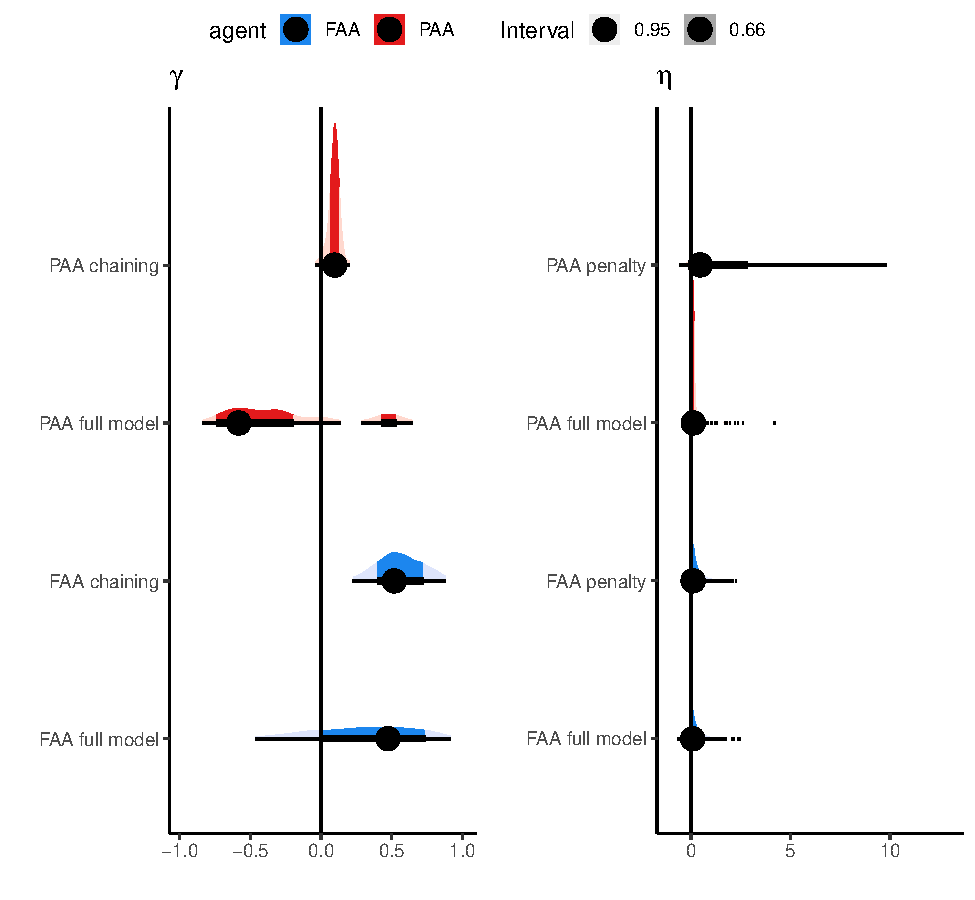
\includegraphics[width=1\linewidth]{manuscript_1.0_files/figure-latex/post-1} 

}

\caption{Posterior distributions for parameter values $\gamma$, $\eta$ and the scaling constant. We show the kernel density estimates, below the mode (black point) and the 65\% (light blue) and 95\% (grey)  highest posterior density interval for the three paramteres. On the left (panels a, c and c) posterior distributions for a model with   all three parameters; while on the right (b and d) a model without negative reward. Panel f shows a measure of fit for both models, namely the distribution of pseudo-$R^2$ obtained from sampling the posterior distribution of parameter values.}\label{fig:post}
\end{figure}

Figure \ref{fig:post} panels a,c and e show the posterior distributions
of the parameter values of the full model, which includes both future
and negative reward. Posterior distributions show the probability
density (y axis) of the estimated parameter values (x axis). Notably,
the bulk of the posterior distribution for the parameter tuning negative
reward (\(\eta\) panel e) is around zero. Thus, the shape of the posterior
and its credible intervals suggest the absence of negative reward to be
well supported by the data. As for \(\gamma\), the confidence intervals
also includes zero, but the mode of the posterior is around 0.5. Thus,
we run the analysis setting \(\eta\) to zero. Figure \ref{fig:post} panels
b and d, show the posterior distributions of the two parameters
estimated. Not surprisingly, under a model without negative reward, the
distribution of \(\gamma\) shifts to higher values. Under the new model,
the estimates of \(\gamma\) do not include zero, the distribution is
centered around \(0.5\). To asses the fit of the two models we calculated
the \(pseudo-R^2\) \citep{mcfadden_Conditional_1974}, which is a standard
measure of fit for logistic regression. In that context, \(pseudo-R^2\)
uses the log-likelihood of the data given the model, relative to the
log-likelihood of the data given a model without covariates, as a
measure of fit. Given that our model is not a logistic regression, we
measure the \(pseudo-R^2\) in relation to the log-likelihood of a model
with parameters \(\gamma\) and \(\eta\) set to zero. This in practice
amounts to a model that has neutral preference between the two options.
In panel f of figure \ref{fig:post} we show the distribution of
\(pseudo-R^2\) calculated using samples from the posterior distributions
shown before, as well as from a model with negative reward but without
future reward. Note, \(pseudo-R^2\) can have negative values, that is when
the log-likelihood of the model is lower than that of a model that
triggers neutral preferences. Even though, the peak of the three
\(pseudo-R^2\) distributions is not very different, the model with only
future reward produces a distribution of \(pseudo-R^2\) where more values
are positive (to the right of black line in Fig. \ref{fig:post} f). This
shows that, accounting for variation in the parameter estimates, the
model with only future reward gives a better fit to the data, despite
having one parameter less.

\begin{figure}

{\centering 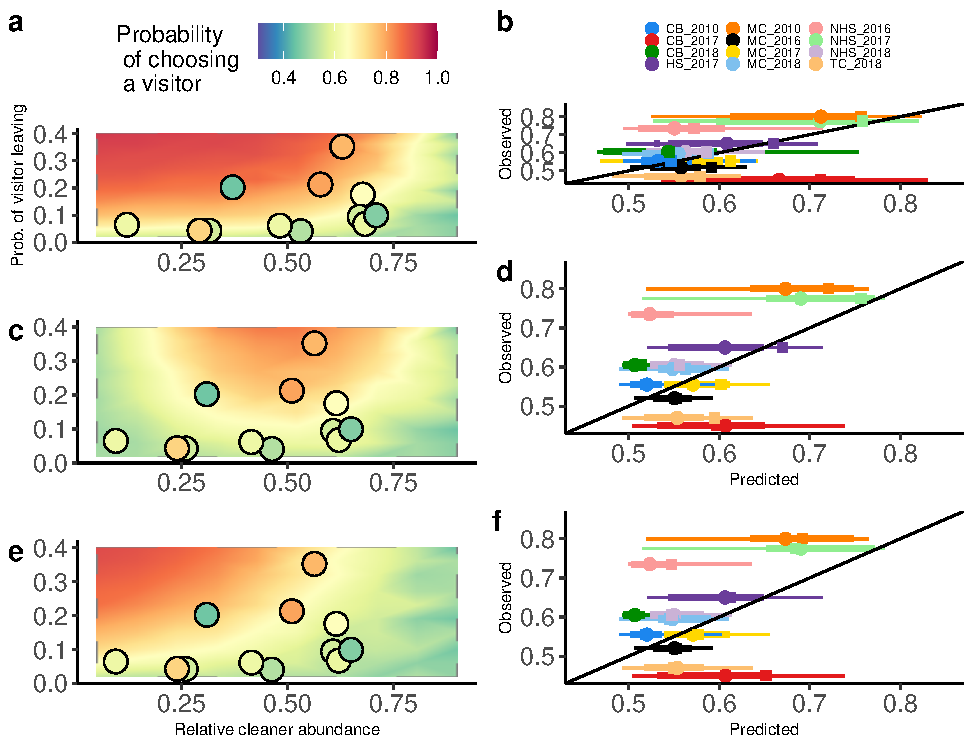
\includegraphics[width=1\linewidth]{manuscript_1.0_files/figure-latex/pred-1} 

}

\caption{Observed and predicted probability of choosing a visitor. Left-hand side panel: color contour shows the prediction of the learning model using the mode of the posterior distributions of parameters recovered by the statistical analysis. Dots show the frequency of visitor choices for the 12 locations, as well as the corresponding relative cleaner abundance (x axis) and frequency of visitors leaving the station (y axis). Right-hand side panels: scatter plot of the observed and predicted probabilities of choosing a visitor for 12 locations. Line correspond to a perfect match between observed and predicted probabilities. Pseudo $R^2$ shown in the lower right corner corresponds to the fit of a model parameterized with the mode of the posterior distributions. Upper panels show prediction from a model including future and negative reward, lower panels froma  model with only future reward.}\label{fig:pred}
\end{figure}

Figure \ref{fig:pred} shows predictions from the two models. On the
left, the colour coded contour shows the prediction of the model for
combinations of cleaner abundance (x axis) and visitor leaving
probability (y axis). Predictions were generated by running the model
using the mode of the posterior distributions as the parameter values,
and varying systematically cleaner abundance and visitor leaving
probability. Colour of the points on top of the contour show the average
frequency with which cleaner fish chose the visitor plate in their last
20 experimental trials. Each point corresponds to a location with a
combination of cleaner abundance and visitor leaving probability. Panels
on the right show how close the observed values for the probability of
choosing the visitor (y axis) are from the predictions of the models (x
axis). The line represents the perfect fit between observed and
predicted values. Predicted values were taken using the mode just as in
the left panels. On the lower right corner of the panel we show the
\(pseudo-R^2\) for predictions using the mode of the posterior
distributions. Despite having one more parameter varying, the full model
gives a lower fit to the data than the model without negative reward.
The difference in \(pseudo-R^2\) for the point estimates is small, but
using the whole posterior distribution shows the improvement in fit
achieved by eliminating negative reward from the model (Fig.
\ref{fig:post}f). In the supplementary material, we also show that a
model with only negative reward, excluding future rewards (\(\gamma=0\),
Fig. \ref{fig:nogamma}), provides a lower fit than either of the ones
presented in the main text.

The main reason for negative and future reward to give different
predictions is the way that cleaner's relative abundance influences the
preference for the visitor clients. Visitor leaving probability has a
similar positive effect on the probability of choosing the visitor
clients on all three models (Fig. \ref{fig:pred}, \ref{fig:nogamma}). In
contrast, cleaner's relative abundance has a different effect in the
model with only future reward, compared to the other two. In the model
with only future reward only intermediate cleaner abundance triggers a
preference for the visitor clients (Fig. \ref{fig:pred} c). In models
with negative reward, both intermediate and low cleaner abundance
trigger a preference for the visitor. (Fig. \ref{fig:pred} a,
\ref{fig:nogamma}).

\hypertarget{discussion}{%
\subsection{Discussion}\label{discussion}}

We have shown that using future rewards in the learning process is the
cognitive strategy that best explains the intra-specific variation in
cleaner performance in the market task. We compared future reward with
the use of visitors behaviour as a primary source of negative reward,
and a combination of both. All three models capture well the positive
relation between visitor leaving behaviour and cleaner performance in
the market task \citep{triki_Biological_2019}. For both mechanisms it is
indeed necessary to have fleeing behaviour on the side of the visitors
for cleaners to develop a preference for them. The key difference
between future and negative reward emerges in the predicted relation
between cleaner relative abundance and cleaner performance. When cleaner
relative abundance is low a model with only future reward predicts low
performance in the market task regardless of the visitor leaving
probability. In contrast, a model with negative reward predicts the
highest performance with low relative cleaner abundance, particularly
together with high probability of visitor leaving (Fig. \ref{fig:pred}).
Low cleaner abundances mean the market has an excess of demand for
cleaning services. In the model, this translates to a cleaning station
that is frequently full. Thus, when visitors leave, it's likely that the
cleaner will have access to another client, and there will not be much
difference in future reward between choosing a visitor and a resident.
Thus, estimation of future reward will not develop a preference for the
visitor in this conditions, because it matches the state of the market.
On the other hand, the effect of negative reward is unaffected by this
market situation. In a full station, cleaners will get more often the
heterotypic (resident-visitor) option and will develop a preference for
the visitor faster. Note that when cleaner abundance is high situations
with a resident and a visitor will be so rare that neither mechanism
will be very efficient in generating a preference for visitors. When
such choice arises it is still be best to choose the visitor; however,
the learning machinery will not be able to develop this preference
efficiently. Overall, estimation of future reward is then the cognitive
mechanism that allows cleaners to adaptively respond conditions to the
ecological conditions of the biological market.

The cognitive mechanism that our analysis highlights does not require a
direct flow of information between the cleaner and its social
environment. The adaptive responses to local conditions in cleaners is
not only evidenced by their performance in experiments, but also by
changes in their brain anatomy. Indeed, individual cleaners that
performed in the laboratory test according to what is best at the
location in which they were caught had larger forebrains harbouring more
cells than individuals whose performance mismatched locally optimal
decision-rules \citep{triki_Brain_2020}. This suggests that despite the
overall behavioural adjustment, evidenced here and elsewhere
\citep{triki_Biological_2019, triki_Decrease_2018}, there are some
cleaners better than others at adjusting their behaviour. Triki \emph{et al.}
\citep{triki_Brain_2020} refer to these as socially competent cleaners. Social
competence refers to the ability to optimise social behaviour depending
on the available social information \citep{taborsky_Social_2012a, bshary_Cooperation_2015}. However, we have shown here that cleaners
are able to adjust their preference according to the social environment
without using any direct information about the social environment.
Instead cleaners seem to adjust their preference using information from
the visitation patterns of their clients. These patters are of course
determined by the feedback with the cleaner's social environment
(relative abundance). Our models, however, do not include the
possibility of cleaners responding to their relative abundance directly.
The mechanism we present is a general way to learn from the environment
in both asocial and social situations. It would be interesting to
contrast this learning mechanism with one tailored to a social
situation, and see whether such mechanism fits the data better. More
generally, an important challenge ahead is to understand which cognitive
mechanisms evolved exclusively for social life.

One potential difference between cleaners that adjusted adaptively, like
the ones reported in Triki \emph{et al.} \citep{triki_Brain_2020}, is configurational learning or
chunking. The original analysis of the learning model showed that agents
needed two mechanism to solve the market task; to account for the
future, and to assign value to the combination of clients present in the
station \citep{quinones_Reinforcement_2019}. The latter is referred to as
configurational learning or chunking \citep{sutherland_Configural_1989, miller_Magical_1956}. Theoretical models suggest that the lack of
configurational learning is related to a low frequency with which
stimuli are encountered together \citep{kolodny_Evolution_2014, prat_Role_2021}. Thus, cleaner relative abundance could be related to
this mechanisms as well. Given that the lack of either of these two
mechanisms yields neutral preferences \citep{quinones_Reinforcement_2019},
we can't, based on the current analysis, distinguish between the two
possibilities. One potential way to distinguish between the two would be
to use an experimental set up designed to test configuration learning on
cleaners with high and low performance in the market task
\citep{woodbury_Learning_1943, sutherland_Configural_1989}.

Combining mechanistic modelling with empirical data provides a powerful
tool to identify the cognitive processes underlying learning in animals.
The combination overcomes the limitations of the general philosophy in
animal cognition to apply the logic of Lloyd Morgen's canon (Occam's
razor). Excluding basic reinforcement learning explanations (operant
and/or classical conditioning) as a potential explanation in experiments
often warrants animals solving the task on the first possible occasion.
For example, any theory of mind task needs to be solved in the first
trial in order to exclude fast conditioning \citep{heyes_Theory_1998}.
Similarly, subjects need to solve a social learning task on the first
trial to accept imitation as a mechanism over stimulus/local
enhancement. Such strict conditions are virtually never met. For
example, potato washing by Japanese macaques, an iconic example of
social learning, took several years to spread within the group
\citep{kawamura_Process_1959}, meaning that any learner had been repeatedly
exposed to demonstrations before acquisition. Importantly, Galef
\citep{galef_Question_1992} refuted imitation as mechanism not simply because
of the repeated exposure but because a (rather qualitative) analysis of
the spread of potato washing across individuals did not follow the
prediction based on imitation learning (see also
\citep{hirata_SweetPotato_2001}). In our case, the number of trials it took
cleaners to learn the solution to the market task would never allow to
exclude an important role of negative reinforcement based on the data
alone. However, fitting model predictions to our data set revealed that
a more complex mechanism (estimation of future reward) fits the data
better.

\newpage

\hypertarget{supplementary-material}{%
\section{Supplementary material}\label{supplementary-material}}

\beginsupplement

\begin{figure}[H]

{\centering 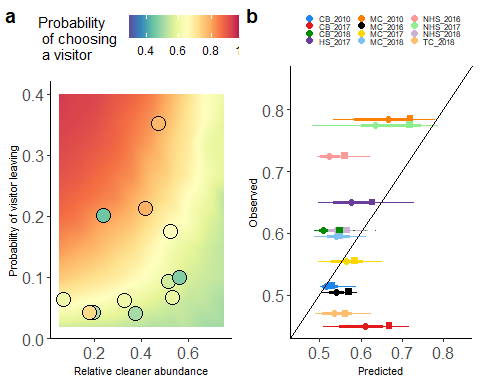
\includegraphics[width=0.95\linewidth,]{manuscript_1.0_files/figure-latex/nogamma-1} 

}

\caption{Observed and predicted probability of choosing a visitor for a model without future rewards. Left-hand side panel: color contour shows the prediction of the learning model using the mode of the posterior distributions of parameters recovered by the statistical analysis. Dots show the frequency of visitor choices for the 12 locations, as well as the corresponding relative cleaner abundance (x axis) and frequency of visitors leaving the station (y axis). Right-hand side panel: scatter plot of the observed and predicted probabilities of choosing a visitor for 12 locations. Line correspond to a perfect match between observed and predicted probabilities.}\label{fig:nogamma}
\end{figure}

\begin{longtable}[]{@{}rc@{}}
\caption{\label{tab:param} Parameter values with which the model was run
in the MCMC. \(\sigma\) refers to the amplitud of the perturbation kernel with the subscript indicating the associated parameter. New values were taken from a uniform distribution. \(\alpha\) refers to the learning rate.}\tabularnewline
\toprule
Parameter & Value \\
\midrule
\endfirsthead
\toprule
Parameter & Value \\
\midrule
\endhead
Learning rounds & 10000 \\
Reward value & 1 \\
\(\alpha\) & 0.05 \\
\(\sigma_{\gamma}\) & 0.3 \\
\(\sigma_{\eta}\) & 4 \\
\(\sigma_{Sca.Const.}\) & 300 \\
Number of chains & 5 \\
Chain lenght & \(1^5\) \\
\bottomrule
\end{longtable}

\ethics{The Animal Ethics Committee of the Queensland government (DAFF)
approved the project (CA 2016/05/970 and CA 2017/05/1063).}

\dataccess{Please provide details on the data availability.}

\aucontribute{AQ and RB designed the study. ZT collected the data. AQ developed the model and
fitted the model parameters to the data. AQ, RB and ZT wrote the manuscript.}

\competing{The authors declate no conflict of interests.}

\funding{This work was supported by the Swiss National Science Foundation (grants
number: 31003A\_153067/1 and 310030B\_173334/1 to R.B.).}


\ack{ZT and RB kindly thank the staff of Lizard Island Research Station, Dominique
Roche, Sharon Wismer, Olivia Rey,Sandra Ann Binning, Elena Levorato and William McNeely for their
field support. AQ thanks Florian Hartig for statistical advice.}

\bibliographystyle{RS}
\bibliography{Cleanerlearning.bib}


\end{document}
